\section{Introduction}
\note{TODO: start visual and interactive data mining more generally?}

Finding multiple ways to characterize the same entities is a problem
that appears in many areas of science. Describing geographical regions in terms of both their
bioclimatic conditions and the fauna that inhabits them is one
instance in the field of biology.  A simple example of a redescription in this setting could
state that areas where Moose live are areas where February's maximum
temperature is between $-10$ and $0$ degrees Celsius and July's
maximum temperature between $12$ and $25$ degrees Celsius.
This is actually the redescription shown in the foreground panel of
Figure~\ref{fig:both_panels}.

\begin{figure*}[t]
  \centering
%%FIG%%
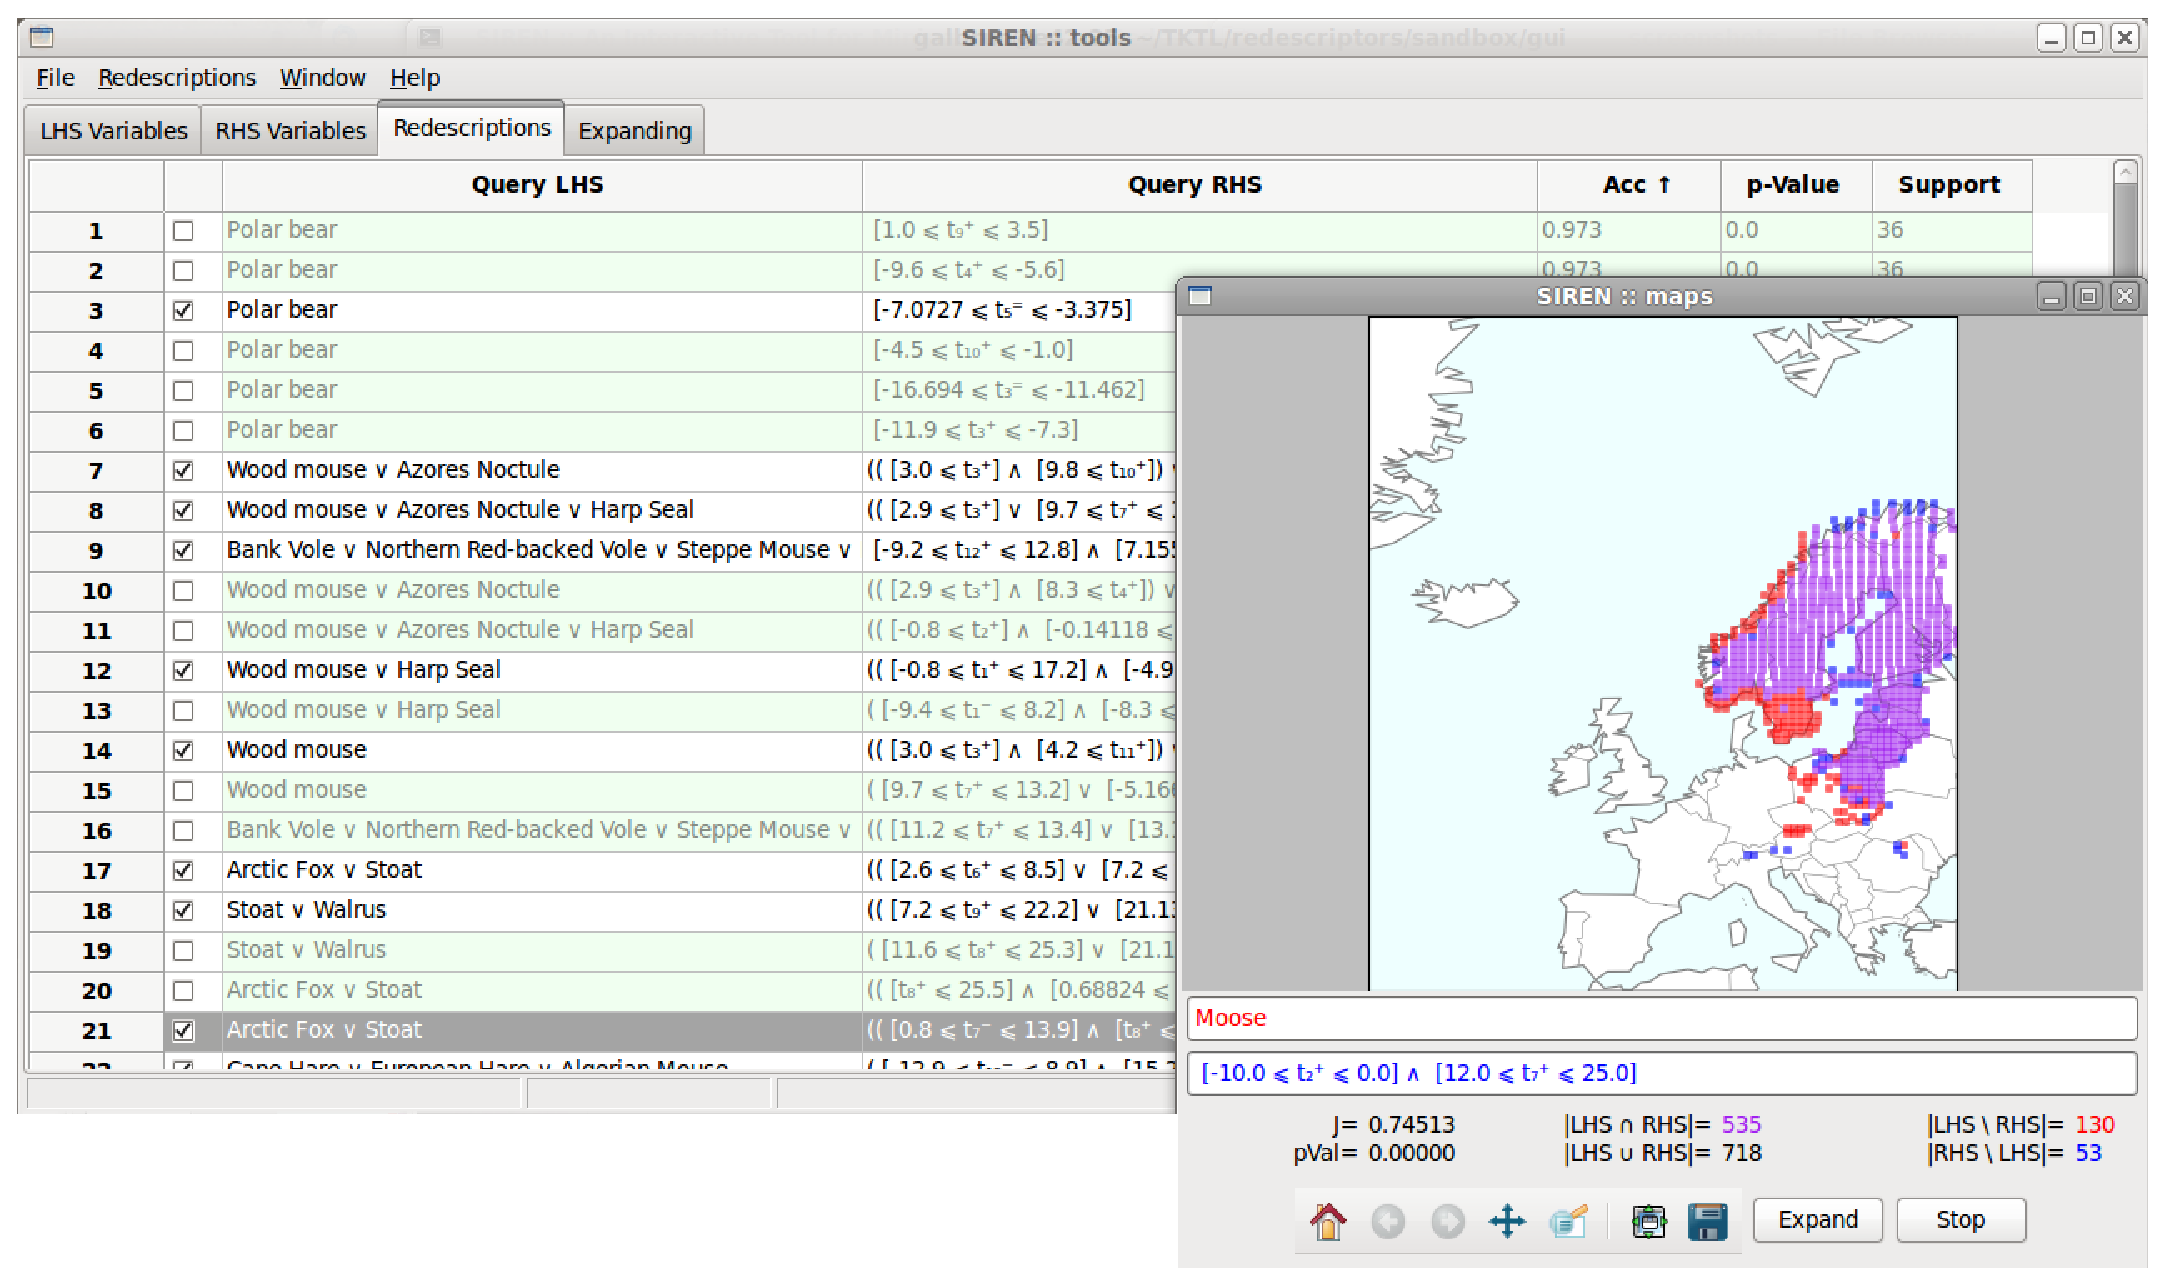
\includegraphics[width=\textwidth]{screenshots/both_panels_02}
  \caption{The \Siren\ interactive mining and visualization tool. The panel in the background contains a list of redescriptions while the foreground panel displays the map of a selected redescription.  In this example, left hand side queries are over fauna while right hand side queries are over monthly bioclimatic conditions, that is, temperatures and precipitation.}
  \label{fig:both_panels}
\end{figure*}

The results of redescription mining, the redescriptions, can be
approached from two points of view. On one hand, by considering the
variables and conditions appearing in the queries, which provide
valuable information in themselves; on the other hand, by studying the
support set of the redescriptions, i.e.\ the subset of entities where
both queries of a redescription hold. 
 
% \note{This explanation is unclear about split between visualization
%   and interactivity and dependance between two.}  \note{But does it
%   matter? I'm not religious about splitting the two -- I don't think
%   it works, in fact -- but I think that presenting the goals with
%   split is easier than in a merry mess of all of them.}  
To analyse the redescriptions, the ability to visualize the support
sets is very helpful. When building a tool for mining redescriptions
from geospatial data, plotting the support on a map, as in the foreground panel of
Figure~\ref{fig:both_panels}, is a natural
visualization. But a static display of the results is not enough: the
user must also be able to interact with the program. This interaction
can be conceptually divided into two sub-phases: interacting with the
data mining algorithm and interacting with the result
visualization. The analysis is an alternation of these two phases,
with the user moving back-and-forth between issuing commands to find
new results and examining obtained ones. We argue that a good
interactive data mining tool should support both types of interaction
and facilitate the alternation between different phases.  

In this paper we give a systematic outline of contributive features to
fulfill that aim, considering the example of mining geospatial
redescriptions. We then present a pair of algorithms, \ReReMi\ and
\Siren, and explain how they implement interactivity and visualization
for that task. Lastly, we discuss some possible pitfalls associated
with interactive, visual mining. But first, we formally define the
redescription mining problem.

%%% Local Variables: 
%%% mode: latex
%%% TeX-master: "siren_iid"
%%% End: 
